% Options for packages loaded elsewhere
\PassOptionsToPackage{unicode}{hyperref}
\PassOptionsToPackage{hyphens}{url}
%
\documentclass[
]{book}
\usepackage{lmodern}
\usepackage{amssymb,amsmath}
\usepackage{ifxetex,ifluatex}
\ifnum 0\ifxetex 1\fi\ifluatex 1\fi=0 % if pdftex
  \usepackage[T1]{fontenc}
  \usepackage[utf8]{inputenc}
  \usepackage{textcomp} % provide euro and other symbols
\else % if luatex or xetex
  \usepackage{unicode-math}
  \defaultfontfeatures{Scale=MatchLowercase}
  \defaultfontfeatures[\rmfamily]{Ligatures=TeX,Scale=1}
\fi
% Use upquote if available, for straight quotes in verbatim environments
\IfFileExists{upquote.sty}{\usepackage{upquote}}{}
\IfFileExists{microtype.sty}{% use microtype if available
  \usepackage[]{microtype}
  \UseMicrotypeSet[protrusion]{basicmath} % disable protrusion for tt fonts
}{}
\makeatletter
\@ifundefined{KOMAClassName}{% if non-KOMA class
  \IfFileExists{parskip.sty}{%
    \usepackage{parskip}
  }{% else
    \setlength{\parindent}{0pt}
    \setlength{\parskip}{6pt plus 2pt minus 1pt}}
}{% if KOMA class
  \KOMAoptions{parskip=half}}
\makeatother
\usepackage{xcolor}
\IfFileExists{xurl.sty}{\usepackage{xurl}}{} % add URL line breaks if available
\IfFileExists{bookmark.sty}{\usepackage{bookmark}}{\usepackage{hyperref}}
\hypersetup{
  pdftitle={Git and GitHub for Reproducible Science},
  pdfauthor={Simona Picardi},
  hidelinks,
  pdfcreator={LaTeX via pandoc}}
\urlstyle{same} % disable monospaced font for URLs
\usepackage{color}
\usepackage{fancyvrb}
\newcommand{\VerbBar}{|}
\newcommand{\VERB}{\Verb[commandchars=\\\{\}]}
\DefineVerbatimEnvironment{Highlighting}{Verbatim}{commandchars=\\\{\}}
% Add ',fontsize=\small' for more characters per line
\usepackage{framed}
\definecolor{shadecolor}{RGB}{248,248,248}
\newenvironment{Shaded}{\begin{snugshade}}{\end{snugshade}}
\newcommand{\AlertTok}[1]{\textcolor[rgb]{0.94,0.16,0.16}{#1}}
\newcommand{\AnnotationTok}[1]{\textcolor[rgb]{0.56,0.35,0.01}{\textbf{\textit{#1}}}}
\newcommand{\AttributeTok}[1]{\textcolor[rgb]{0.77,0.63,0.00}{#1}}
\newcommand{\BaseNTok}[1]{\textcolor[rgb]{0.00,0.00,0.81}{#1}}
\newcommand{\BuiltInTok}[1]{#1}
\newcommand{\CharTok}[1]{\textcolor[rgb]{0.31,0.60,0.02}{#1}}
\newcommand{\CommentTok}[1]{\textcolor[rgb]{0.56,0.35,0.01}{\textit{#1}}}
\newcommand{\CommentVarTok}[1]{\textcolor[rgb]{0.56,0.35,0.01}{\textbf{\textit{#1}}}}
\newcommand{\ConstantTok}[1]{\textcolor[rgb]{0.00,0.00,0.00}{#1}}
\newcommand{\ControlFlowTok}[1]{\textcolor[rgb]{0.13,0.29,0.53}{\textbf{#1}}}
\newcommand{\DataTypeTok}[1]{\textcolor[rgb]{0.13,0.29,0.53}{#1}}
\newcommand{\DecValTok}[1]{\textcolor[rgb]{0.00,0.00,0.81}{#1}}
\newcommand{\DocumentationTok}[1]{\textcolor[rgb]{0.56,0.35,0.01}{\textbf{\textit{#1}}}}
\newcommand{\ErrorTok}[1]{\textcolor[rgb]{0.64,0.00,0.00}{\textbf{#1}}}
\newcommand{\ExtensionTok}[1]{#1}
\newcommand{\FloatTok}[1]{\textcolor[rgb]{0.00,0.00,0.81}{#1}}
\newcommand{\FunctionTok}[1]{\textcolor[rgb]{0.00,0.00,0.00}{#1}}
\newcommand{\ImportTok}[1]{#1}
\newcommand{\InformationTok}[1]{\textcolor[rgb]{0.56,0.35,0.01}{\textbf{\textit{#1}}}}
\newcommand{\KeywordTok}[1]{\textcolor[rgb]{0.13,0.29,0.53}{\textbf{#1}}}
\newcommand{\NormalTok}[1]{#1}
\newcommand{\OperatorTok}[1]{\textcolor[rgb]{0.81,0.36,0.00}{\textbf{#1}}}
\newcommand{\OtherTok}[1]{\textcolor[rgb]{0.56,0.35,0.01}{#1}}
\newcommand{\PreprocessorTok}[1]{\textcolor[rgb]{0.56,0.35,0.01}{\textit{#1}}}
\newcommand{\RegionMarkerTok}[1]{#1}
\newcommand{\SpecialCharTok}[1]{\textcolor[rgb]{0.00,0.00,0.00}{#1}}
\newcommand{\SpecialStringTok}[1]{\textcolor[rgb]{0.31,0.60,0.02}{#1}}
\newcommand{\StringTok}[1]{\textcolor[rgb]{0.31,0.60,0.02}{#1}}
\newcommand{\VariableTok}[1]{\textcolor[rgb]{0.00,0.00,0.00}{#1}}
\newcommand{\VerbatimStringTok}[1]{\textcolor[rgb]{0.31,0.60,0.02}{#1}}
\newcommand{\WarningTok}[1]{\textcolor[rgb]{0.56,0.35,0.01}{\textbf{\textit{#1}}}}
\usepackage{longtable,booktabs}
% Correct order of tables after \paragraph or \subparagraph
\usepackage{etoolbox}
\makeatletter
\patchcmd\longtable{\par}{\if@noskipsec\mbox{}\fi\par}{}{}
\makeatother
% Allow footnotes in longtable head/foot
\IfFileExists{footnotehyper.sty}{\usepackage{footnotehyper}}{\usepackage{footnote}}
\makesavenoteenv{longtable}
\usepackage{graphicx,grffile}
\makeatletter
\def\maxwidth{\ifdim\Gin@nat@width>\linewidth\linewidth\else\Gin@nat@width\fi}
\def\maxheight{\ifdim\Gin@nat@height>\textheight\textheight\else\Gin@nat@height\fi}
\makeatother
% Scale images if necessary, so that they will not overflow the page
% margins by default, and it is still possible to overwrite the defaults
% using explicit options in \includegraphics[width, height, ...]{}
\setkeys{Gin}{width=\maxwidth,height=\maxheight,keepaspectratio}
% Set default figure placement to htbp
\makeatletter
\def\fps@figure{htbp}
\makeatother
\setlength{\emergencystretch}{3em} % prevent overfull lines
\providecommand{\tightlist}{%
  \setlength{\itemsep}{0pt}\setlength{\parskip}{0pt}}
\setcounter{secnumdepth}{5}
\usepackage{booktabs}
\usepackage[]{natbib}
\bibliographystyle{apalike}

\title{Git and GitHub for Reproducible Science}
\author{Simona Picardi\footnote{Utah State University, \href{mailto:simona.picardi@usu.edu}{\nolinkurl{simona.picardi@usu.edu}}}}
\date{2021-09-13}

\begin{document}
\maketitle

{
\setcounter{tocdepth}{1}
\tableofcontents
}
\hypertarget{overview}{%
\chapter{Overview}\label{overview}}

The goal of this workshop is to teach you how to efficiently manage and share
your code. Code is a living, ever-changing thing, and using it efficiently
requires a system able to accommodate changes implemented through time and by
multiple users while guaranteeing long-term integrity. Version control is a
powerful tool to help us achieve efficient code management, and more broadly,
reproducible research. Here, we will focus on Git and GitHub as our software of
choice. At the end of these two days, you will be able to:

\begin{enumerate}
\def\labelenumi{\arabic{enumi}.}
\tightlist
\item
  Optimize your directory organization;
\item
  Create Git repositories for each of your research projects;
\item
  Automatically keep track of changes you make in your code;
\item
  Synchronize changes between collaborators on a project;
\item
  Retrieve previous versions of code when necessary.
\end{enumerate}

The content is organized in two Chapters, articulated over two days:

\begin{itemize}
\tightlist
\item
  Chapter \ref{version-control-git}, Version Control with Git
\item
  Chapter \ref{git-hub}, Collaborative Science with GitHub
\end{itemize}

\hypertarget{software-requirements-and-installation-instructions}{%
\section{Software Requirements and Installation Instructions}\label{software-requirements-and-installation-instructions}}

\hypertarget{git}{%
\subsection{Git}\label{git}}

Git is a distributed version control system. It is free and open source. To
install Git, follow instructions for your operating system below.

\hypertarget{windows}{%
\subsubsection{Windows}\label{windows}}

Download from the Git website: go to \url{https://git-scm.com/download/win} and the
download will start automatically.

\hypertarget{mac-os}{%
\subsubsection{Mac OS}\label{mac-os}}

On Mavericks (10.9) or above, when you try to run a Git command from the
Terminal for the first time, the installation will start automatically if you
don't already have Git installed. Type the following in the terminal:

\begin{Shaded}
\begin{Highlighting}[]

\NormalTok{$ }\FunctionTok{git}\NormalTok{ --version}
\end{Highlighting}
\end{Shaded}

And follow the instructions on the installation wizard.

\hypertarget{linux}{%
\subsubsection{Linux}\label{linux}}

In the command line:

\begin{Shaded}
\begin{Highlighting}[]

\NormalTok{$ }\FunctionTok{sudo}\NormalTok{ apt install git-all}
\end{Highlighting}
\end{Shaded}

\hypertarget{github}{%
\subsection{GitHub}\label{github}}

We are going to use GitHub through the web browser, so no need to install any
additional software. Just make sure you create a GitHub account on \url{https://github.com/}.

\hypertarget{version-control-git}{%
\chapter{Version Control with Git}\label{version-control-git}}

Git is a version control system. It tracks all the changes you make to your files and allows you to go back to previous versions as far back in time as you need, like a time machine. Git is useful for a variety of reasons. Most of us are familiar with folders that look like this:

\begin{figure}
\centering
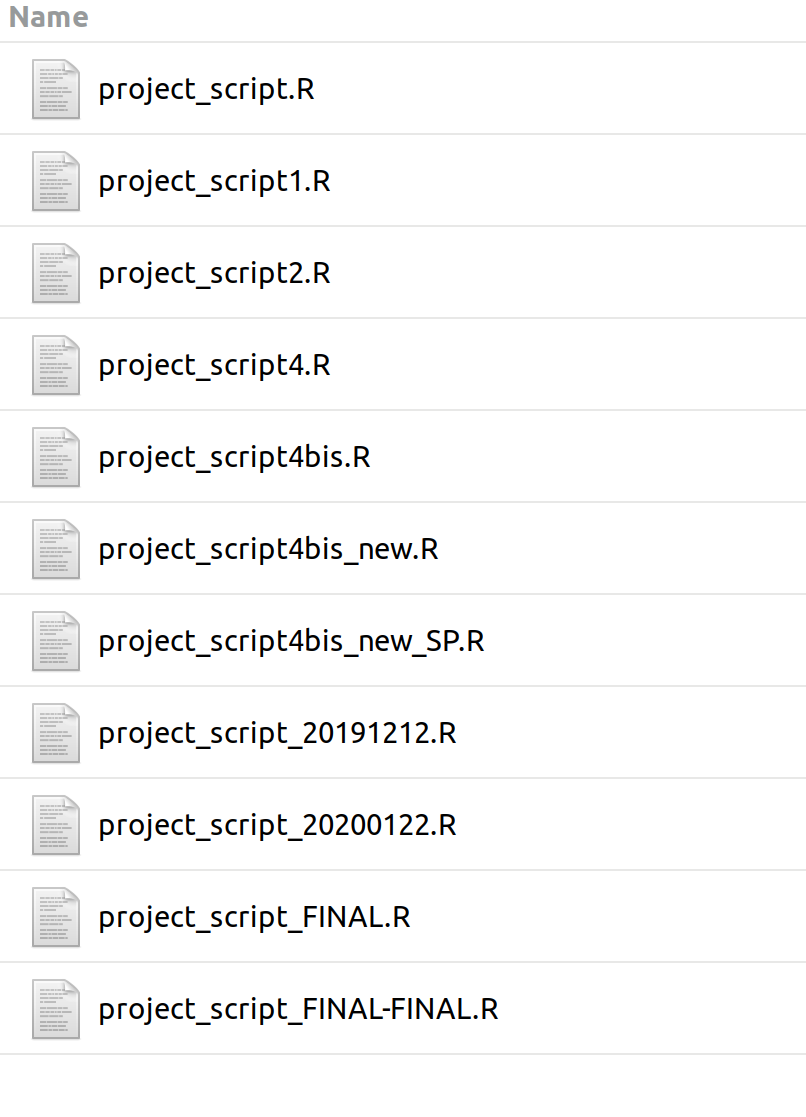
\includegraphics[width=0.5\textwidth,height=\textheight]{img/version-nightmare.png}
\caption{Messy folder}
\end{figure}

Saving multiple versions of files like this is problematic because, first, it uses space inefficiently (even if files are small, multiple versions add up and end up wasting a lot of room on our computers); second, and perhaps most importantly, it creates confusion and makes our workflow prone to errors. Instead of manually saving edits to a file in a separate copy ``just in case'', and instead of having to keep track of which is the most recent version, we can put our files under version control and let Git keep track of the changes we make. Git will record a history of changes to each file without duplicating it, and we'll be able to revert to any previous version in the history of that file. Version control allows us to be clean and tidy in our file organization, optimizing use of space without ever fearing to lose any of our work. Once a file is tracked by Git, it is virtually impossible to do anything irreversible to it.

I haven't mentioned anything yet about the benefits of version control for collaborative work. This is because at its core, Git works locally on your computer. We often tend to think of version control as the way to handle multiple users working on the same file simultaneously, but Git is first and foremost a tool for your own file organization. Git is installed and runs on your machine, not on a network. It is the integration with an external server, be it private or public (GitHub and GitLab, for example, are public server providers), that makes Git a tool for multiple-user applications. This chapter focuses on the local functionalities of Git, while we'll dive into its benefits for collaborative projects in the next Chapter.

\hypertarget{directory-organization}{%
\section{Directory organization}\label{directory-organization}}

Git works on a project-by-project basis. Each project you work on with Git will become its own \textbf{Git repository}. A repository is nothing but a folder with Git functionalities enabled on it. Because everything in Git revolves around repositories as functional units, deciding how to split our files into folders will make the difference between a smooth, streamlined workflow and a clunky, inefficient one. So, to make the most of Git, we need to take a step back and take a look at how files are organized on our computer.

Your file browser, or file explorer, shows your directory tree (directory is a synonym for folder). The base of the tree is what we call the root directory (this is usually \texttt{C:/} in Windows and \texttt{/} on Mac/Linux). Nested folders and subfolders branch out from the root and define our directory structure. There are infinite possible directory structures that we can choose to organize our files. For example, say that we are working on a research project that entails data cleaning, analysis, and writing of a manuscript. One way to go about it is to have a project directory that contains subfolders for data, analysis code, results, and the manuscript file/s. We can call this a ``project-based directory layout.''

\begin{figure}

{\centering 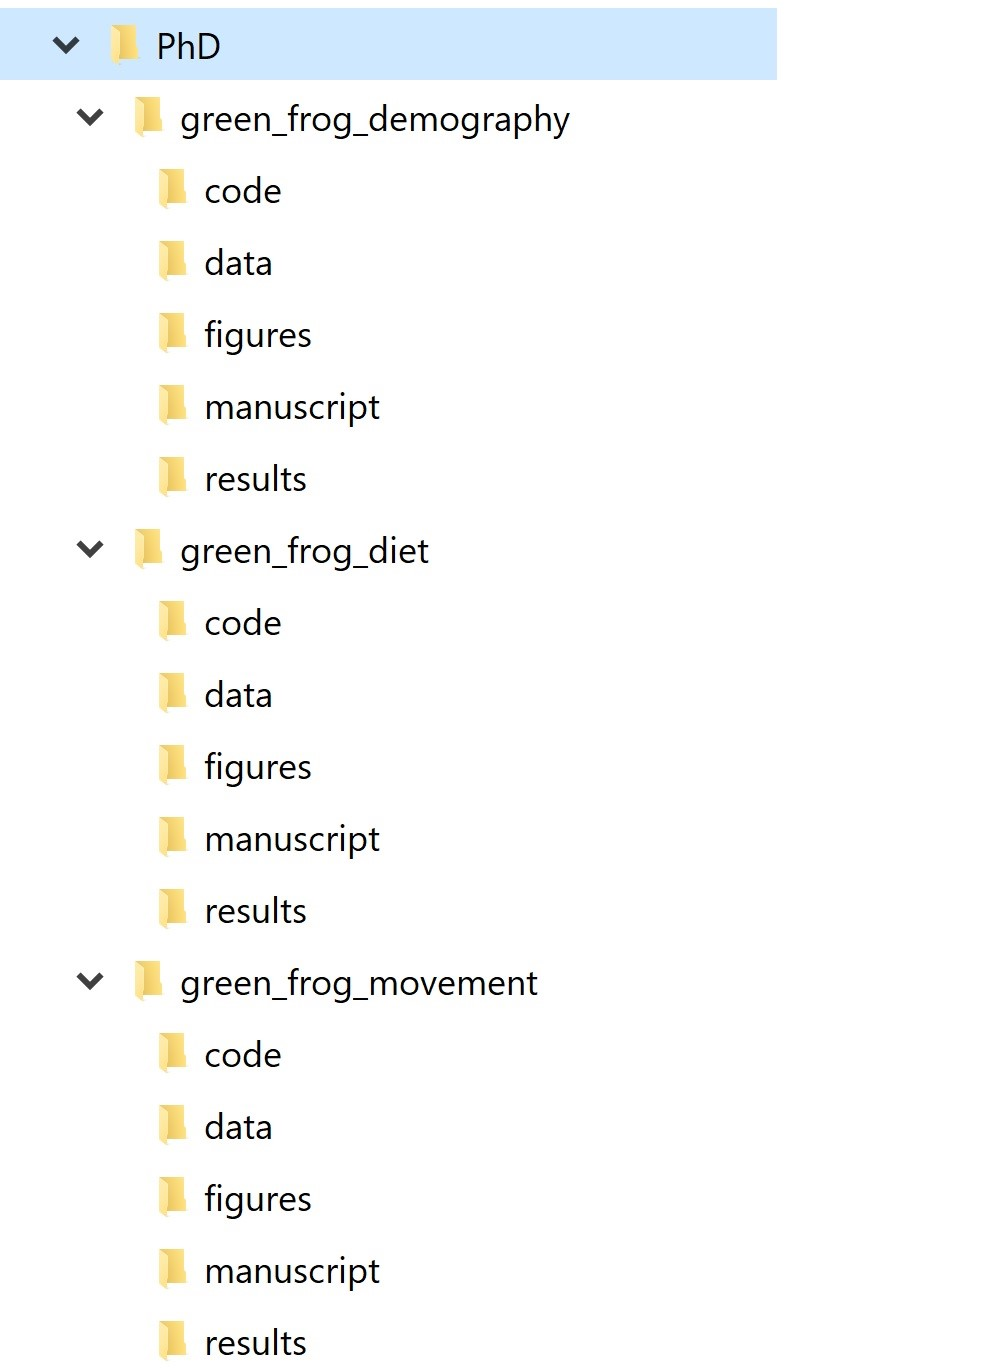
\includegraphics[width=0.5\linewidth]{img/project-based-directory-organization} 

}

\caption{Project-based directory organization}\label{fig:proj-based}
\end{figure}

Alternatively, if we have multiple projects underway, we can split our files by activity rather than by projects and have a ``data'' folder, an ``analyses'' folder, a ``manuscripts'' folder, etc., all with a subfolder for each project. We can call this an ``activity-based directory layout.''

\begin{figure}

{\centering 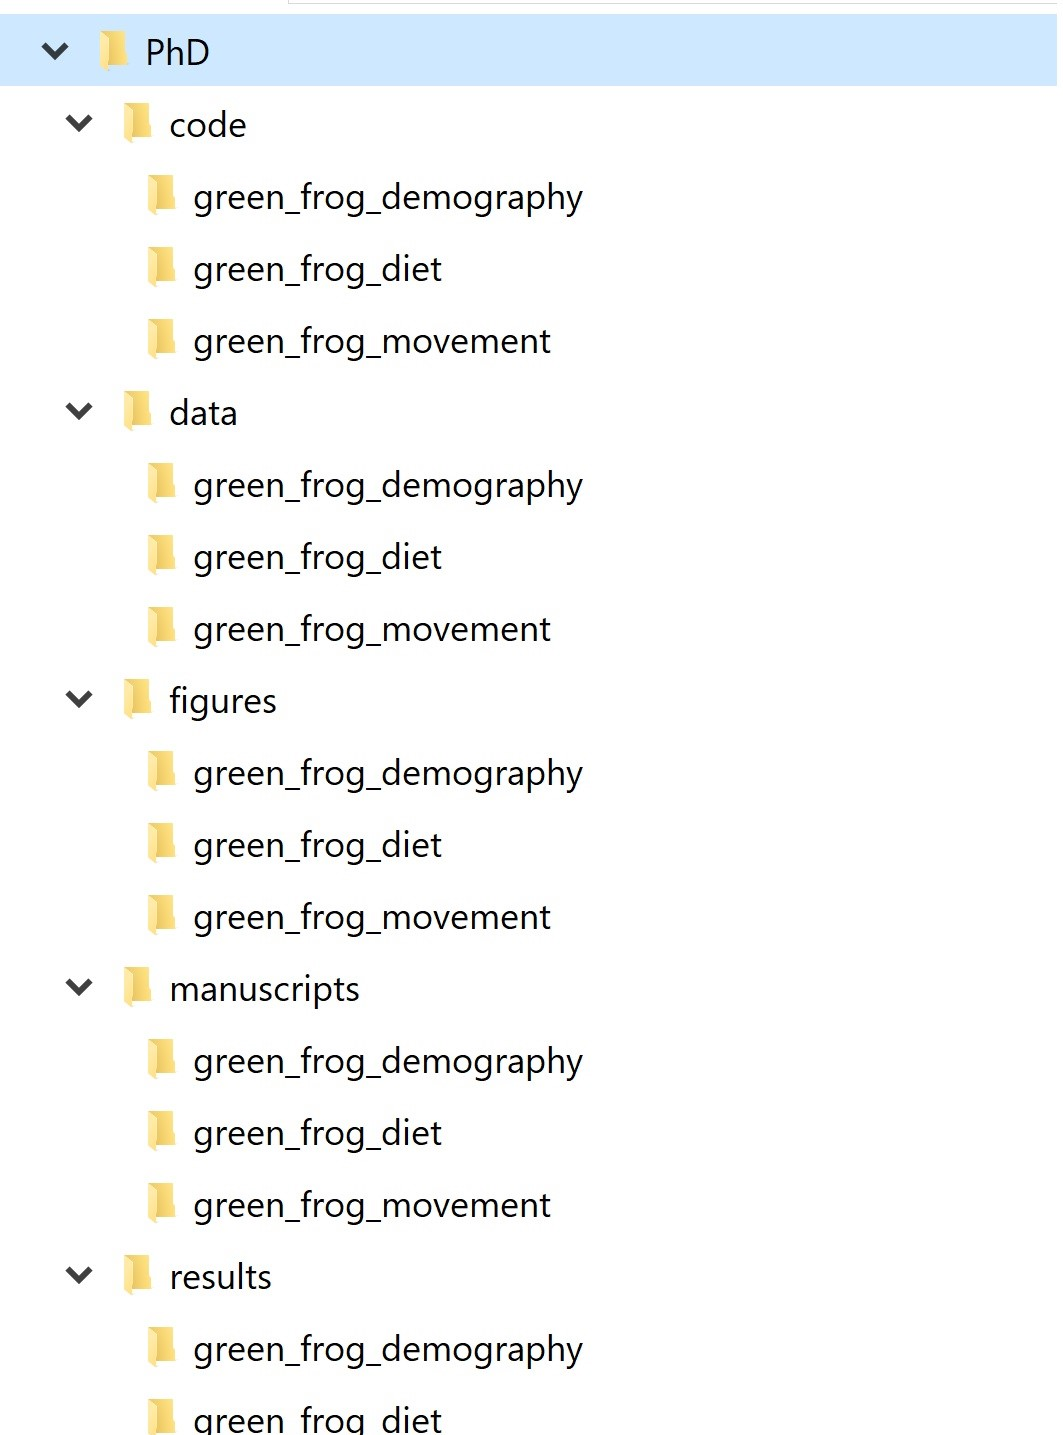
\includegraphics[width=0.5\linewidth]{img/activity-based-directory-organization} 

}

\caption{Activity-based directory organization}\label{fig:act-based}
\end{figure}

How you define a project is largely up to you. It could be all the work you do on a given dataset, or all the work you do for a thesis or dissertation, or each manuscript could be its own project even if it uses the same dataset as a different project. With so many options, how do we choose? Here are some key criteria to keep in mind:

\hypertarget{overlap}{%
\subsection{Overlap}\label{overlap}}

The first thing to consider is the overlap in data and code files between a project and other past/current projects. If two projects don't share any data, it's probably best to manage them separately. If two projects share a large amount of data, it might make more sense to manage them together as one. If you are writing functions to use across several different projects, they should probably be in their own project.

\hypertarget{minimizing-duplication}{%
\subsection{Minimizing duplication}\label{minimizing-duplication}}

The reason why it's important to account for overlap is because you want to minimize duplication as much as you can. Duplication of both data and code files is dangerous because it's easy to lose track of modifications you have made to a file saved in one place but not in the other place. As you keep making changes, the two files will have the same name but different content, which generates confusion. Duplication is also inefficient because it occupies precious space on your computer.

\hypertarget{self-containedness}{%
\subsection{Self-containedness}\label{self-containedness}}

A fundamental quality of reproducible projects is that they are self-contained, meaning that ideally you could zip up the entire project directory and send it to a friend and they should be able to run your code and reproduce your results without changing anything. This means everything the project needs to work, from A to Z -- data, functions, code -- is contained in its root directory.

\hypertarget{tradeoffs}{%
\subsection{Tradeoffs}\label{tradeoffs}}

The self-containedness criterion is sometimes in contradiction with minimizing duplication: if two projects share one or more data files, you can either violate the duplication criterion by making sure each project contains all the necessary data for the sake of self-containedness; or you can choose to sacrifice self-containedness to avoid file duplication and save space on your computer. The answer will depend on whether you anticipate the project to be widely shared or mostly for your personal use, how large the shared data files are, etc.

The bottom line is that there is no one-size-fits-all solution for project organization. Most importantly, the structure you choose needs to be functional for your needs. Putting thought into it is a great place to start.

\hypertarget{golden-rules-for-file-organization}{%
\section{Golden rules for file organization}\label{golden-rules-for-file-organization}}

Whichever directory structure you choose for a project, there are some universal rules to keep in mind for how to organize files within it.

\begin{enumerate}
\def\labelenumi{\arabic{enumi}.}
\item
  First and foremost, \textbf{raw data should never be changed}. Save it into a ``data'' folder and treat it as immutable. You can even set it as read-only to make sure there is no room for accidents.
\item
  The processed, clean version of your data will go into a dedicated ``processed\_data'' folder.
\item
  Anything that can be generated from code goes into its own folder. This includes basically everything but the raw data and the code itself. You can have an ``output'' folder, or separate folders for output files and figures (e.g., ``output'' and ``figures'')
\item
  If there are text documents, put them in their own folder (e.g., ``docs'')
\item
  Code also has its own folder. If you write a lot of functions, it can be helpful to have a ``funs'' folder to store those and a ``src'' (for `source') folder to save processing/analysis code.
\item
  If processing/analysis scripts are meant to be used in a certain order, you can number them (more on this in a minute). Sometimes the pipeline is not linear but branched, so numbering may not always make sense. Function scripts should not be numbered.
\item
  Modularize your code: instead of having a giant script to run your entire analysis from data cleaning to final figures, break up your workflow into several short, single-purpose scripts with well-defined inputs and outputs.
\end{enumerate}

\hypertarget{relative-and-absolute-paths}{%
\section{Relative and absolute paths}\label{relative-and-absolute-paths}}

To efficiently use Git, it is important to feel comfortable navigating our computer using paths. Paths define the location of files within the file system. There are two ways to point to a file from within a command prompt. The first is to use what is called an absolute path: this describes the full sequence of folders a file is contained in, starting from the root directory of a computer. When you right click on any file on your computer, you can look up its absolute path in the Properties. This is an example of an absolute path:

\begin{quote}
C:/Users/MJS/Documents/PhD/Planning/schedule\_2021.csv
\end{quote}

Relative paths describe the position of a file with respect to a reference directory. The reference directory is called a ``working directory''. A relative path only shows the way from the working directory to the file of interest, while the part that goes from the root to the reference directory is left implicit. Appending a relative file path to the path of the working directory gives us the full absolute path to that file. For example, if our working directory was ``Documents'', this would be the relative path to reach the same file as above:

\begin{quote}
PhD/Planning/schedule\_2021.csv
\end{quote}

If our working directory was ``Planning'', this would be the relative path to the same file:

\begin{quote}
schedule\_2021.csv
\end{quote}

To work across subfolders of our working directory, we can just use relative paths to navigate and locate files. But relative paths also work to navigate across folders that are outside of the working directory, if need be. Using ``../'' in front of a folder name navigates to the parent of that folder (``parent'' means the folder where that is contained). Let's consider the following directory structure:

\begin{figure}

{\centering 
\includegraphics[width=32in]{img/directory-tree} 

}

\caption{Example directory structure}\label{fig:dir-example}
\end{figure}

We can navigate to a file into ``PhD/Research'' from ``Planning'' like so:

\begin{quote}
../Research/GreenFrogs/data-cleaning.RProj
\end{quote}

The ``../'' means ``the parent directory of the working directory'', which is ``PhD''. We can also stack these to navigate further up the directory tree:

\begin{quote}
../../../../DAJ
\end{quote}

The path above navigates all the way up to ``Users'' and into a different user's directory.

\hypertarget{path-separators}{%
\subsection{Path separators}\label{path-separators}}

Something to be mindful of is that the separator between folder names in a path is different on different operating systems. On Windows, it is a backslash (``\textbackslash{}''), while on Mac/Linux, it is a slash (``/'').

\hypertarget{command-line-basics}{%
\section{Command line basics}\label{command-line-basics}}

We are going to use Git from the command line in the computer's terminal. The command line can be intimidating if you haven't used it before, but using Git only requires basic familiarity with it. Commands are slightly different between operating systems, so I'll assume Windows is the most commonly used and specify the Mac/Linux alternative when applicable.

When you open up the terminal (or command prompt) on your computer, you'll see a symbol, on many computers it is a ``\$'' or ``\textgreater{}'', followed by a blinking cursor. That symbol is called the prompt, and it means the terminal is waiting for your input. If you copy-paste any code from this chapter into your terminal,
\textbf{make sure you only copy the part after the prompt} (don't copy the \textgreater).
Also, if Ctrl+V does not work in the terminal, you can right-click to paste.

When you open the terminal, you should automatically be located in the root directory of your file system (or your home directory, if you have a computer with multiple users). The name of the folder you're in appears right before the prompt. For example, this is what my prompt looks like:

\begin{Shaded}
\begin{Highlighting}[]
\OperatorTok{>} \ExtensionTok{C}\NormalTok{:\textbackslash{}Users\textbackslash{}Simona}\OperatorTok{>}
\end{Highlighting}
\end{Shaded}

If you are not in your root directory when you first open up the terminal, you can use the following command to navigate to it:

\begin{Shaded}
\begin{Highlighting}[]
\OperatorTok{>} \BuiltInTok{cd}\NormalTok{ \textbackslash{}}
\end{Highlighting}
\end{Shaded}

This command stands for ``change directory''. The ``\textbackslash{}'' symbol indicates the root directory. On Mac/Linux, you can navigate to the root directory by simply typing ``cd'' or:

\begin{Shaded}
\begin{Highlighting}[]
\OperatorTok{>} \BuiltInTok{cd}\NormalTok{ ~}
\end{Highlighting}
\end{Shaded}

If you want to go to a specific directory other than the root, you can type its path (relative to the folder you're currently in) after ``cd''. To go from Users\textbackslash Simona to Users\textbackslash Simona\textbackslash Documents:

\begin{Shaded}
\begin{Highlighting}[]
\OperatorTok{>} \BuiltInTok{cd}\NormalTok{ Documents}
\end{Highlighting}
\end{Shaded}

If you want to go back to the parent of the current directory (the folder that contains it), you can use:

\begin{Shaded}
\begin{Highlighting}[]
\OperatorTok{>} \BuiltInTok{cd}\NormalTok{ ..}
\end{Highlighting}
\end{Shaded}

To go back to Users from Documents:

\begin{Shaded}
\begin{Highlighting}[]
\OperatorTok{>} \BuiltInTok{cd}\NormalTok{ ..\textbackslash{}..}
\end{Highlighting}
\end{Shaded}

To go back to Documents from Users:

\begin{Shaded}
\begin{Highlighting}[]
\OperatorTok{>} \BuiltInTok{cd}\NormalTok{ Simona\textbackslash{}Documents}
\end{Highlighting}
\end{Shaded}

\hypertarget{configuring-git}{%
\section{Configuring Git}\label{configuring-git}}

Once Git is installed on our computer, we need to do a few one-time steps to configure it. Let's set up our name and our email address by typing the following in the terminal:

\begin{Shaded}
\begin{Highlighting}[]
\OperatorTok{>} \FunctionTok{git}\NormalTok{ config --global user.name }\StringTok{"First Last"}
\OperatorTok{>} \FunctionTok{git}\NormalTok{ config --global user.email }\StringTok{"first.last@example.com"}
\end{Highlighting}
\end{Shaded}

This will be important when we start using GitHub. If you want to change these options in the future you always can, and if you want to use different options than the global ones within a specific project you can run the commands above removing ``--global'' while in the project directory (not the root!).

There are more configuration options you can personalize, but we won't get into that in this workshop. If you want to check what configuration options you have active, you can use:

\begin{Shaded}
\begin{Highlighting}[]
\OperatorTok{>} \FunctionTok{git}\NormalTok{ config --list}
\end{Highlighting}
\end{Shaded}

\hypertarget{getting-help}{%
\section{Getting help}\label{getting-help}}

If you need help while using Git, you can use any of the following commands to get the manual page for any of the Git verbs:

\begin{Shaded}
\begin{Highlighting}[]
\OperatorTok{>} \FunctionTok{git}\NormalTok{ help }\OperatorTok{<}\NormalTok{verb}\OperatorTok{>}
\OperatorTok{>} \FunctionTok{git} \OperatorTok{<}\NormalTok{verb}\OperatorTok{>}\NormalTok{ --help}
\OperatorTok{>} \FunctionTok{man}\NormalTok{ git-}\OperatorTok{<}\NormalTok{verb}\OperatorTok{>}
\end{Highlighting}
\end{Shaded}

\hypertarget{creating-a-repository}{%
\section{Creating a repository}\label{creating-a-repository}}

Once Git is set up and configured, we are ready to create our first repository. A repository is a directory that is under version control. Let's use the example directory structure from Figure \ref{fig:dir-example}. First, we navigate to the folder where we want to initialize our repository. In our example's case, that is:

\begin{Shaded}
\begin{Highlighting}[]
\OperatorTok{>} \BuiltInTok{cd}\NormalTok{ Documents\textbackslash{}PhD\textbackslash{}Research\textbackslash{}GreenFrogs}
\end{Highlighting}
\end{Shaded}

Now we will enable Git to start tracking everything inside this folder:

\begin{Shaded}
\begin{Highlighting}[]
\OperatorTok{>} \FunctionTok{git}\NormalTok{ init}
\end{Highlighting}
\end{Shaded}

This command initializes Git. It may appear like nothing changed, but if you allow the option to show hidden files in your file explorer you will notice there is a new subfolder called .git. That folder is where Git will store all of its version control information. You don't have to worry about the content of that folder and you can keep using your files normally like you always would.

\hypertarget{tracking-files}{%
\section{Tracking files}\label{tracking-files}}

Creating a repository enables Git to start tracking files within it, but that does not happen automatically. We have to tell Git which files we want to track. We can check what Git is tracking so far by using:

\begin{Shaded}
\begin{Highlighting}[]
\OperatorTok{>} \FunctionTok{git}\NormalTok{ status }
\end{Highlighting}
\end{Shaded}

At the bottom, we'll see a list of untracked files. We need to switch on tracking on those. To begin tracking a new file, we use the verb `add'. For example, to track a file named ``green\_frog\_diet\_data\_cleaning.R'' we would type:

\begin{Shaded}
\begin{Highlighting}[]
\OperatorTok{>} \FunctionTok{git}\NormalTok{ add green_frog_diet_data_cleaning.R}
\end{Highlighting}
\end{Shaded}

This works well if we want to add a specific file. If we want to start tracking the whole content of the folder, we can do:

\begin{Shaded}
\begin{Highlighting}[]
\OperatorTok{>} \FunctionTok{git}\NormalTok{ add --all}
\end{Highlighting}
\end{Shaded}

But be careful when using this command: Git is optimized to work with plain text files (for example .txt or R scripts), and it doesn't really understand binary files (which is how Word files are stored, for example). Also, some files typically do not need to be version controlled, such as images; in fact, because they are large files, version controlling images can end up clogging your workflow. Make sure you are always aware of what exactly you're adding when you use `git add --all'. When in doubt, add files one by one. There are also ways to make this process a little more distraction-proof: in the next step, we'll see how to make sure we only track the files we want.

\hypertarget{ignoring-files}{%
\section{Ignoring files}\label{ignoring-files}}

We can set up some rules to exclude from version control files that it would be superfluous or detrimental to track. Writing these down as rules can save us some time and headaches versus having to decide manually every time. We can exclude files from version control within a repository by using .gitignore. This is simply a text file that lists all the rules for files that, by default, we do not want to track. Rules can be based on the file type or patterns in the file name. Generally, there are a few criteria you can consider when deciding what to exclude from version control:

\begin{itemize}
\tightlist
\item
  File encoding (plain-text vs.~binary): Git cannot track changes within binary files, so, even though you \textbf{can} store these files under version control, you won't be able to use Git to compare different version, so there's really no point in tracking these;
\item
  Code-generated: anything that can be reproduced by running code does not need to be version-controlled;
\item
  Size: files that are too big will slow down the functioning of Git. As a benchmark, you can keep in mind the maximum size limit enforced by GitHub, which is 100 MB -- but if you follow the two criteria above, you will rarely end up with this problem because 100 MB's worth of plain-text files is a whole lot of plain text.
\end{itemize}

You can create a text file called ``.gitignore'' in our repository by using your default text editor (Notepad for Windows, TextEdit for MacOS, etc). The name must be exactly ``.gitignore'' for Git to recognize it. The file must have no extension (i.e., .txt) so go ahead and delete that (don't worry about any warnings).

Once .gitignore is created, we can start adding rules. Nothing prevents us from listing files in .gitignore one by one, but this approach is not efficient:

\begin{quote}
stacked\_barplot\_diet\_composition.jpg\\
predicted\_population\_trends.jpg\\
individual\_movement\_tracks.jpg\\
capture\_locations.jpg\\
green\_frog\_diet\_manuscript.docx\\
green\_frog\_movement\_manuscript.docx\\
green\_frog\_demography\_manuscript.docx
\end{quote}

Instead, we can use pattern matching to kill many birds with one stone. What all these files have in common is they are all either .jpg's or .docx's. We can use the wildcard '*' to signify ``any character'' before the file extension:

\begin{quote}
*.jpg\\
*.docx
\end{quote}

This will exclude any .jpg or .docx file from being tracked by Git in this repository. Since the images are conveniently located all together in one folder, we can also just do this:

\begin{quote}
figures/
\end{quote}

We should also add the following rules to ignore the user-specific R project files:

\begin{quote}
*.Rhistory\\
/.Rproj.user/
\end{quote}

We can add as many rules as we like, then save the .gitignore text file when we're done. Now, if we didn't forget to include anything that needed to be ignored, we can safely add all our files in one go:

\begin{Shaded}
\begin{Highlighting}[]
\OperatorTok{>} \FunctionTok{git}\NormalTok{ add --all}
\end{Highlighting}
\end{Shaded}

\hypertarget{the-3-states}{%
\section{The 3 states}\label{the-3-states}}

Once files are tracked by Git, they can be in one of three states: modified, staged, or committed. A modified file includes edits that have not been recorded in Git yet; when we stage a modified file, we mark it as ready to be committed; when we commit that staged file, the current version gets stored in the history of that file.

Git works with snapshots called ``commits'', which are records of what the repository looked like at a certain point in time. By committing a file, we freeze that version of the file forever in its history and we will be able to go back to it. Then, if we edit the file again, we'll have to tell Git when we're ready to make a new commit by moving that file to the staging area. Note that the same command \texttt{git\ add} is used both to start tracking a previously untracked file and to add a modified file to the staging area.

Now we are ready to do our first commit. We use the following command:

\begin{Shaded}
\begin{Highlighting}[]
\OperatorTok{>} \FunctionTok{git}\NormalTok{ commit -m }\StringTok{"First commit"}
\end{Highlighting}
\end{Shaded}

Each commit should be accompanied by a message, added with the flag \texttt{-m}. The message should describe the changes made to the file/s since the previous commit. It is a good habit to write detailed commit messages, so that when we need to go back and recover a previous version of a file, we can read the history of commits and easily find the version we are looking for.

\hypertarget{un-staging-files}{%
\section{Un-staging files}\label{un-staging-files}}

It happens to the best of us. We forgot to add a certain rule to .gitignore and when we go ahead and get ready to commit our files we realized we just staged a file we didn't want to stage. No worries, there is a way to fix that. The following command un-stages files and saves us from having to commit them:

\begin{Shaded}
\begin{Highlighting}[]
\OperatorTok{>} \FunctionTok{git}\NormalTok{ rm --cached filename}
\end{Highlighting}
\end{Shaded}

You can use pattern matching here as well, but you'll need to put a backslash in front of the wildcard:

\begin{Shaded}
\begin{Highlighting}[]
\OperatorTok{>} \FunctionTok{git}\NormalTok{ rm --cached }\DataTypeTok{\textbackslash{}*}\NormalTok{.jpg}
\end{Highlighting}
\end{Shaded}

\hypertarget{recovering-a-previous-version-of-a-file}{%
\section{Recovering a previous version of a file}\label{recovering-a-previous-version-of-a-file}}

Git works like a time machine, allowing us to recover any previous version of a tracked file. It does so by saving snapshots of what the file looked like at each commit. So, each commit represent a point in time that we can access to retrieve the version that existed at that time. We can take a look at the commit history using:

\begin{Shaded}
\begin{Highlighting}[]
\OperatorTok{>} \FunctionTok{git}\NormalTok{ log}
\end{Highlighting}
\end{Shaded}

Here's where current me will be grateful to past me for writing descriptive commit messages. If the commit messages do a good job of describing what changes I made to a file, it will be easy to recognize which commit is the one I want to go back to.

The string of numbers and letters following the word `commit' in the log is called the hash and it uniquely identifies each commit. We can revert to the version of a file from a specific commit by using the hash as follows:

\begin{Shaded}
\begin{Highlighting}[]
\OperatorTok{>} \FunctionTok{git}\NormalTok{ checkout 9c5d9a3f52b7d43c1c0a06a94b11df5c3051ca27 -- filename.ext}
\end{Highlighting}
\end{Shaded}

\hypertarget{removing-git}{%
\section{Removing Git}\label{removing-git}}

If for any reason you ever want to remove Git tracking from a repository (going back to a regular folder without version control) you can use the following command:

\begin{Shaded}
\begin{Highlighting}[]
\OperatorTok{>} \FunctionTok{rm}\NormalTok{ -rf .git}
\end{Highlighting}
\end{Shaded}

\hypertarget{git-everyday}{%
\section{Git everyday}\label{git-everyday}}

This chapter walked you through commands to configure git, initialize repositories, stage and un-stage files, commit changes, and revert to previous versions of a file. In practice, you may use some of these commands only once (e.g., to configure your email address when you first install Git) or when you start a new repository. In your everyday use of Git, the most important commands you need to remember are those to add and commit your changes. For everything else, feel free to refer back to this manual or other resources on the internet.

\hypertarget{references}{%
\section{References}\label{references}}

\begin{itemize}
\tightlist
\item
  Wilson G, Bryan J, Cranston K, Kitzes J, Nederbragt L, Teal TK (2017) Good enough practices in scientific computing. PLoS Comput Biol 13(6): e1005510. \url{https://doi.org/10.1371/journal.pcbi.1005510}
\item
  R for Data Science by Hadley Wickham and Garrett Grolemund: \url{https://r4ds.had.co.nz/workflow-projects.html}
\item
  The Carpentries lesson on Version Control with Git: \url{http://swcarpentry.github.io/git-novice/}
\item
  Pro Git by Scott Chacon and Ben Straub: \url{https://git-scm.com/book/en/v2}
\end{itemize}

\hypertarget{git-hub}{%
\chapter{Collaborative Science with GitHub}\label{git-hub}}

Yesterday we have gained a good understanding of how Git works locally on our computer. Today we are going to see how to work with remote repositories and use Git to collaborate with others. A remote repository is a copy of a repository that is stored elsewhere than your local copy, such as a web server or a private network server. In most cases, when collaborating, you'll have a copy of a repository on your machine (the local repository) and a copy on a server that is accessible to others (the remote repository). The remote repository can be hosted on GitHub. By making sure changes are synchronized between local and remote copies of a repository, we can ensure each collaborator on a project is always working with the most recent version.

There are two ways to set up your local and remote repositories to interact. One is to set up the local first and link it with a remote later. The second one is to create the remote first and ``clone it'' on your computer to get a local copy. If you're starting a brand new repository you can go either way, but the first approach is what you would do if you wanted to link a repository that already exists on your local machine to a GitHub repository.

\hypertarget{adding-a-remote-to-a-local-repository}{%
\section{Adding a remote to a local repository}\label{adding-a-remote-to-a-local-repository}}

Starting from an existing Git repository on your computer, you can link this to its GitHub counterpart by adding a remote URL. To set up a URL, go on the GitHub website, click on the `+' sign in the top-right corner and select `New Repository'.

\begin{figure}

{\centering 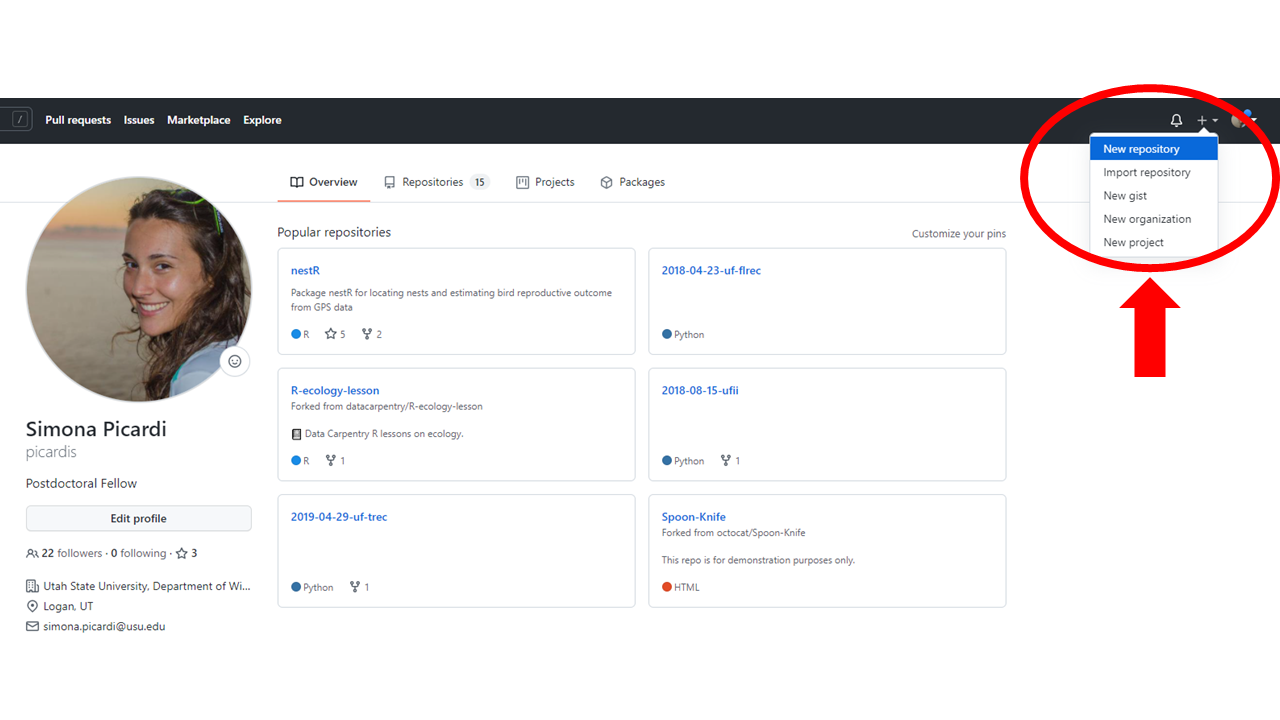
\includegraphics[width=1\linewidth]{img/github-01} 

}

\caption{Create new GitHub repository}\label{fig:github01}
\end{figure}

You can choose any name for your repository, but I find it intuitive to give it the same name as the folder where my local Git repository is. Since the remote repository will need to be connected to a local one, it needs to be completely empty: if there are conflicts in the content of the two repositories to begin with, Git won't be able to link them. Therefore, do not add a README, a .gitignore file, or a license.

\begin{figure}

{\centering 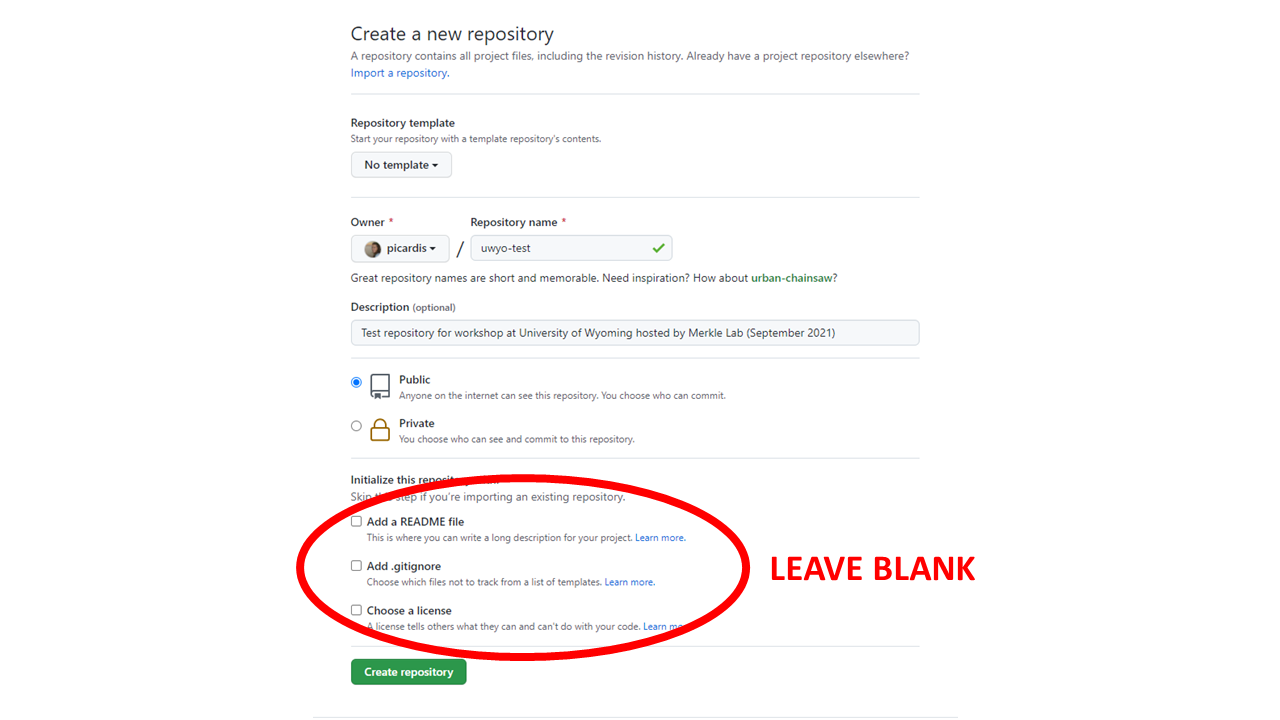
\includegraphics[width=1\linewidth]{img/github-02} 

}

\caption{Create new GitHub repository}\label{fig:github02}
\end{figure}

To connect the local and remote repositories, you can copy the URL of the remote repository and paste it in the following command in the terminal:

\begin{Shaded}
\begin{Highlighting}[]
\OperatorTok{>} \FunctionTok{git}\NormalTok{ remote add origin https://github.com/picardis/myrepo.git}
\end{Highlighting}
\end{Shaded}

`Origin' is the conventional name given to a remote repository. You could use any other name, but since GitHub uses `origin' as the default name when creating a repository from the website, using this convention will make things easier later. You'd need a very good reason to use a different name.

To check that the remote was added correctly you can view the list of remotes associated with your local repository:

\begin{Shaded}
\begin{Highlighting}[]
\OperatorTok{>} \FunctionTok{git}\NormalTok{ remote -v}
\end{Highlighting}
\end{Shaded}

We'll talk about branches later in this chapter, and we'll see that a repository can have multiple branches. At a minimum, each repository includes one main branch, which is created by default when you create your repository. By default, this branch is called \texttt{master}. Starting in 2020, GitHub has started to switch to using \texttt{main} instead of \texttt{master} to remove unnecessary references to slavery. We like this change, because Black Lives Matter. So we'll go ahead and rename the \texttt{master} branch to \texttt{main}:

\begin{Shaded}
\begin{Highlighting}[]
\OperatorTok{>} \FunctionTok{git}\NormalTok{ branch -M main}
\end{Highlighting}
\end{Shaded}

\hypertarget{pushing-to-a-remote-repository}{%
\section{Pushing to a remote repository}\label{pushing-to-a-remote-repository}}

Now it's time to transfer an exact copy of the files in the local repository to the remote one. This action is called `pushing'. The first time you push, it's a good idea to specify which branch Git should use as the default remote for the local main branch in the future. We do this by adding the flag `-u' (for upstream), followed by the name of the remote and the name of the local branch that you want to link up:

\begin{Shaded}
\begin{Highlighting}[]
\OperatorTok{>} \FunctionTok{git}\NormalTok{ push -u origin main}
\end{Highlighting}
\end{Shaded}

This command is identical to the following:

\begin{Shaded}
\begin{Highlighting}[]
\OperatorTok{>} \FunctionTok{git}\NormalTok{ push --set-upstream origin main}
\end{Highlighting}
\end{Shaded}

You only have to set the upstream the first time you push a certain branch. After the upstream is set up, you will be able to just push changes to the remote repository by doing:

\begin{Shaded}
\begin{Highlighting}[]
\OperatorTok{>} \FunctionTok{git}\NormalTok{ push}
\end{Highlighting}
\end{Shaded}

You will be prompted to enter your GitHub password for the push to go through.

Once you push, all the files you committed are transferred and your two repositories will mirror each other. To keep the remote repository synchronized with the local, any time you commit changes to tracked files you will also need to push them. That adds a new step to our workflow: add/stage, commit, push.

\hypertarget{cloning-a-repository}{%
\section{Cloning a repository}\label{cloning-a-repository}}

The other way to get a local-remote repository pair set up is to create a GitHub repository first and clone it on your computer. In this case, it doesn't matter whether the remote repository is empty or not, so you can add a README. Cloning a repository is also useful if you are collaborating on a project with someone on their repository. You and your collaborator/s can all have a copy of the same repository on each of your computers by cloning a shared remote repository, which will then be synchronized with changes made by anyone on the team. The person who created the repository will need to add the others as collaborators so that they're able to clone it.

To clone a repository, open the terminal and navigate to the folder where you want to download it. Then use the following command:

\begin{Shaded}
\begin{Highlighting}[]
\NormalTok{$ }\FunctionTok{git}\NormalTok{ clone https://github.com/picardis/myrepo.git}
\end{Highlighting}
\end{Shaded}

The repository will be copied to your computer into the folder you specified.

\hypertarget{synchronizing-changes-among-collaborators}{%
\section{Synchronizing changes among collaborators}\label{synchronizing-changes-among-collaborators}}

The inverse of pushing is pulling, which transfers files and changes from the remote repository to the local one:

\begin{Shaded}
\begin{Highlighting}[]
\NormalTok{$ }\FunctionTok{git}\NormalTok{ pull }
\end{Highlighting}
\end{Shaded}

When you are working with collaborators on a shared GitHub repository, you will periodically need to pull from it to make sure your local copy is synchronized with changes somebody else might have made. You certainly need to pull before you push your own changes, because Git won't allow you to push if the remote repository has changes that you don't have on your local copy. If the two repositories are already up-to-date and you try to pull, nothing will happen because there are no changes on the remote repository that aren't already in the local.

If a collaborator makes a change that is in conflict with what we committed to our own local repository, when we try to pull we are going to encounter a merge conflict. Merge conflicts occur when two collaborators work on the same file at the same time. GitHub does not know how to automatically reconcile changes to the same file, and it will throw an error that we'll need to resolve manually.

\hypertarget{resolving-conflicts}{%
\section{Resolving conflicts}\label{resolving-conflicts}}

Having to deal with merge conflicts is eventually very likely when working on collaborative projects, but they can be handled and resolved without too much pain.

If two collaborators edit the same file at the same time without pulling each other's changes first, when one tries to push their changes to the remote they will get an error message that looks like this:

\begin{Shaded}
\begin{Highlighting}[]
\ExtensionTok{To}\NormalTok{ https://github.com/picardis/myrepo.git}
\NormalTok{ ! [}\ExtensionTok{rejected}\NormalTok{]        master -}\OperatorTok{>}\NormalTok{ master (fetch first)}
\ExtensionTok{error}\NormalTok{: failed to push some refs to }\StringTok{'https://github.com/picardis/myrepo.git'}
\ExtensionTok{hint}\NormalTok{: Updates were rejected because the remote contains work that you do}
\ExtensionTok{hint}\NormalTok{: not have locally. This is usually caused by another repository pushing}
\ExtensionTok{hint}\NormalTok{: to the same ref. You may want to first integrate the remote changes}
\ExtensionTok{hint}\NormalTok{: (e.g., }\StringTok{'git pull ...'}\NormalTok{) }\ExtensionTok{before}\NormalTok{ pushing again.}
\ExtensionTok{hint}\NormalTok{: See the }\StringTok{'Note about fast-forwards'}\NormalTok{ in }\StringTok{'git push --help'}\NormalTok{ for details.}
\end{Highlighting}
\end{Shaded}

Git is rejecting the push because it found some updates in the remote repository that have not been incorporated in the local copy. To solve this, the person who got the error will need to pull the most recent changes, merge them into their current copy, and then push the resulting file.

After pulling, if we open the file where the conflict is, we'll find that Git did not erase one person's changes in favor of the other's; instead, it marked the lines where conflicting changes occur. The beginning and end of the problematic chunk are highlighted, and the two versions are separated by `=' signs.

Now it is up to us to reconcile these changes however we consider appropriate. We could keep our own changes, keep the changes made by our collaborator, write something new to replace both, or delete the change entirely. Once the conflict is removed and the file is saved, we can proceed as usual by staging the file, committing it, and pushing it. Now, when any of the other collaborators pulls from the repository again, they will get the merged version of this file.

In some cases, collaborators will make simultaneous changes to a file that are mutually exclusive -- for example, one person will delete a line of code while another person will edit that same line. However, changes don't need to be mutually exclusive for a merge conflict to happen: any time two users edit the same line of the same file at the same time (for example, two users may both add a new argument to the same function), Git is going to play it safe and call a merge conflict regardless of whether the changes contradict each other or not. Conflict resolution requires the user to verify whether the changes affect each other and if they can both stay or not.

\hypertarget{avoiding-conflicts}{%
\section{Avoiding conflicts}\label{avoiding-conflicts}}

Merge conflicts need to be manually resolved by a person, which is time-consuming. More importantly, the person who resolves a merge conflicts is making a judgement call on what is the best way of fixing the situation. Having to introduce subjective judgement calls is perhaps the weakest spot of the entire collaborative version control workflow. Preventing conflicts from happening in the first place is better than having to fix them. There are a few things that can help prevent merge conflicts:

\begin{itemize}
\tightlist
\item
  Pull often: decreases probability that your working version is not up-to-date;
\item
  Make small and frequent commits: decreases probability that your recent changes are not in other people's working version;
\item
  Organize your code in small modules: decreases probability of two users working on the same file;
\item
  Working on branches or forks\ldots{} more on this in the next sections.
\end{itemize}

\hypertarget{working-with-branches}{%
\section{Working with branches}\label{working-with-branches}}

By default, a new repository contains a single branch: the main branch. However, we can create new branches within a repository. A branch is like a parallel universe where any changes we make on the files only exist on that branch and do not affect the main branch. Branches allow you to freely experiment with editing files and code without affecting the original project until you're ready to merge them.

The command to create a branch is:

\begin{Shaded}
\begin{Highlighting}[]
\OperatorTok{>} \FunctionTok{git}\NormalTok{ branch my-branch}
\end{Highlighting}
\end{Shaded}

To start working on the new branch, we switch to it with the following command:

\begin{Shaded}
\begin{Highlighting}[]
\OperatorTok{>} \FunctionTok{git}\NormalTok{ checkout my-branch}
\end{Highlighting}
\end{Shaded}

Or we could also create the branch and switch to it all in one:

\begin{Shaded}
\begin{Highlighting}[]
\OperatorTok{>} \FunctionTok{git}\NormalTok{ checkout -b my-branch}
\end{Highlighting}
\end{Shaded}

Where ``b'' stands for branch. To verify which branch we're on, we can use `git log' (we've used this same command before to look at the commit history):

\begin{Shaded}
\begin{Highlighting}[]
\OperatorTok{>} \FunctionTok{git}\NormalTok{ log }
\end{Highlighting}
\end{Shaded}

The word `HEAD' in the output of \texttt{git\ log} is called a pointer; it tells us which branch we're currently working on. On creation, a new branch shares the commit history of the main branch up until the moment the branch was created. After that, the two commit histories are allowed to diverge. Any changes we commit to a branch will be only effective on the that branch and not affect the others. This takes off all the pressure of making changes to your code that could potentially break your workflow downstream. Once you've had a chance to verify that the changes work the way you want them to, you can merge the branches back into one.

To merge changes made in a branch into the main branch we use:

\begin{Shaded}
\begin{Highlighting}[]
\OperatorTok{>} \FunctionTok{git}\NormalTok{ merge my-branch}
\end{Highlighting}
\end{Shaded}

And then we can delete the `my-branch' branch which is no longer needed:

\begin{Shaded}
\begin{Highlighting}[]
\NormalTok{$ }\FunctionTok{git}\NormalTok{ branch -d my-branch}
\end{Highlighting}
\end{Shaded}

If there are conflicting changes on the two branches we are trying to merge, Git will halt the process and issue a merge conflict similar to what we have seen before.

\hypertarget{forking-a-repository}{%
\section{Forking a repository}\label{forking-a-repository}}

Forking a repository means creating a copy of an existing repository where you can make changes without affecting the original repository. You can technically fork your own repository, but forking is mostly used to get a copy of somebody else's repository. For example, if you want to contribute to a project that was created by a person you don't know, or if you want to build off of their code because it does something similar to what you need to do, you can fork their repository and work on it without their copy being affected.

The cool thing about forking is that, if the owner makes changes to their repository, you can pull those changes to your fork so that your copy of the repository stays in sync with the original. Also, you can contribute your own changes by submitting them to the original repository through pull requests. This is the main difference between forking and cloning somebody else's repository: by cloning, you won't be able to update your copy to include new changes made in the original and you won't be able to contribute back unless you're added as a collaborator.

Unlike all the other functionalities we have seen so far, which are Git commands, forking is a GitHub functionality. There is no built-in Git function to fork a repository from the command line. To fork a repository, go to the web page of that repository and click ``Fork'' in the top-right corner. This will create a copy of the repository on your GitHub account.

\begin{figure}

{\centering 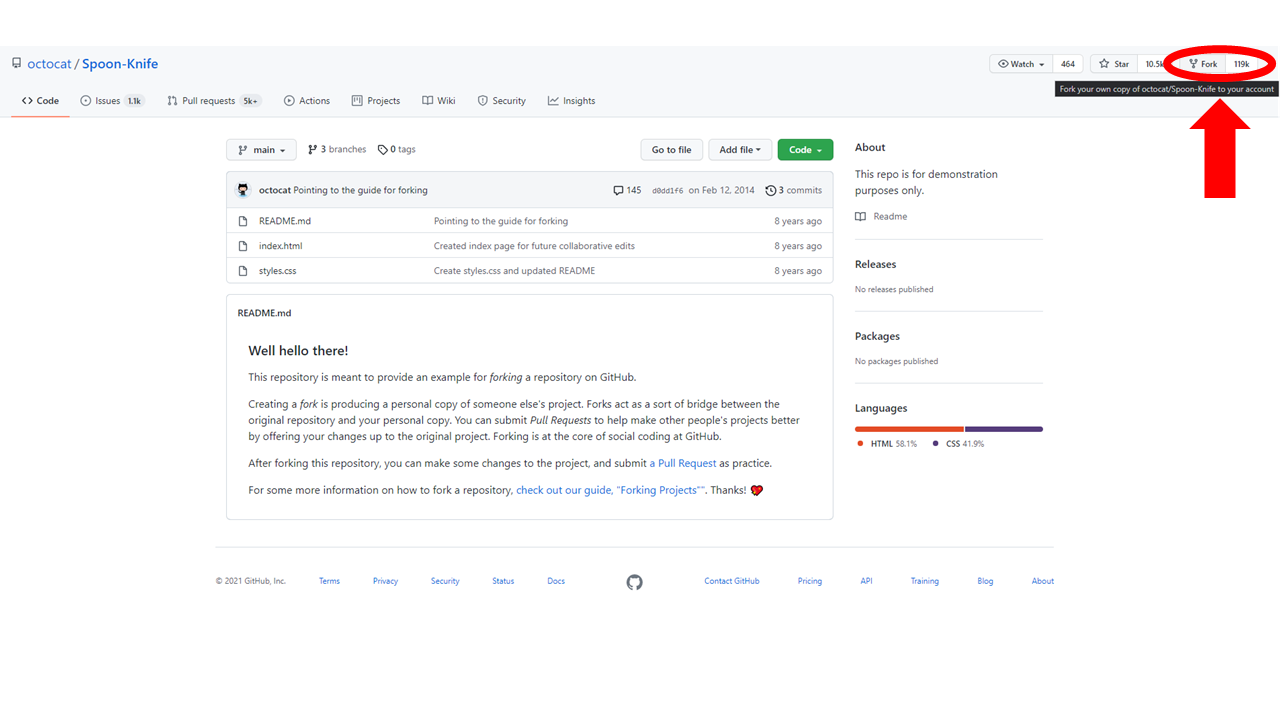
\includegraphics[width=1\linewidth]{img/github-03} 

}

\caption{Fork GitHub repository}\label{fig:github03}
\end{figure}

Now, if you also want a local copy of this repository on your computer, you can clone your fork. For example, if I forked octocat's Spoon-Knife repository onto my GitHub account, I could then clone it onto my computer like so:

\begin{Shaded}
\begin{Highlighting}[]
\OperatorTok{>} \FunctionTok{git}\NormalTok{ clone https://github.com/picardis/Spoon-Knife}
\end{Highlighting}
\end{Shaded}

To keep my fork up-to-date with the original repository, I can configure it as follows:

\begin{Shaded}
\begin{Highlighting}[]
\NormalTok{$ }\FunctionTok{git}\NormalTok{ remote add upstream https://github.com/octocat/Spoon-Knife.git}
\end{Highlighting}
\end{Shaded}

Now I will be able to pull from the original repository and keep my local copy synchronized. I won't be able to push because I do not have collaborator privileges on this repository.

\hypertarget{pull-requests}{%
\section{Pull requests}\label{pull-requests}}

Pull requests are the way to ask that the edits you made in a fork (or a branch) get merged into the original repository (or main branch). To ask the owner of a repository to view and potentially integrate the changes you made in your own forked version, you submit a pull request. Similarly, to let your collaborators know about the edits you made and let them review them before they get merged, you submit a pull request. There is a key difference here: while as an external agent you have no other choice but submitting a pull request to merge a fork into a repository, as a collaborator you could simply merge your edits if you wanted to. If you are working on your own repository by yourself, there is no need to go through pull requests to merge a branch. But if you are collaborating with people, it is still good and courteous practice to use pull requests as a heads-up before you merge your changes, so that others on the project can review and approve them.

The most straightforward way to submit a pull request is from the GitHub website. To start a pull request, you must have some changes committed to the repository or branch where you want to merge them. Then you can go to the repository page on GitHub and click on the `Pull requests' tab, then click `New pull request'. Choose your target branch, enter a title and description, and then click `Send pull request'. Once the pull request is open, everyone can write comments on it, see all the commits it includes, and look at the changes it proposes within files.

\begin{figure}

{\centering 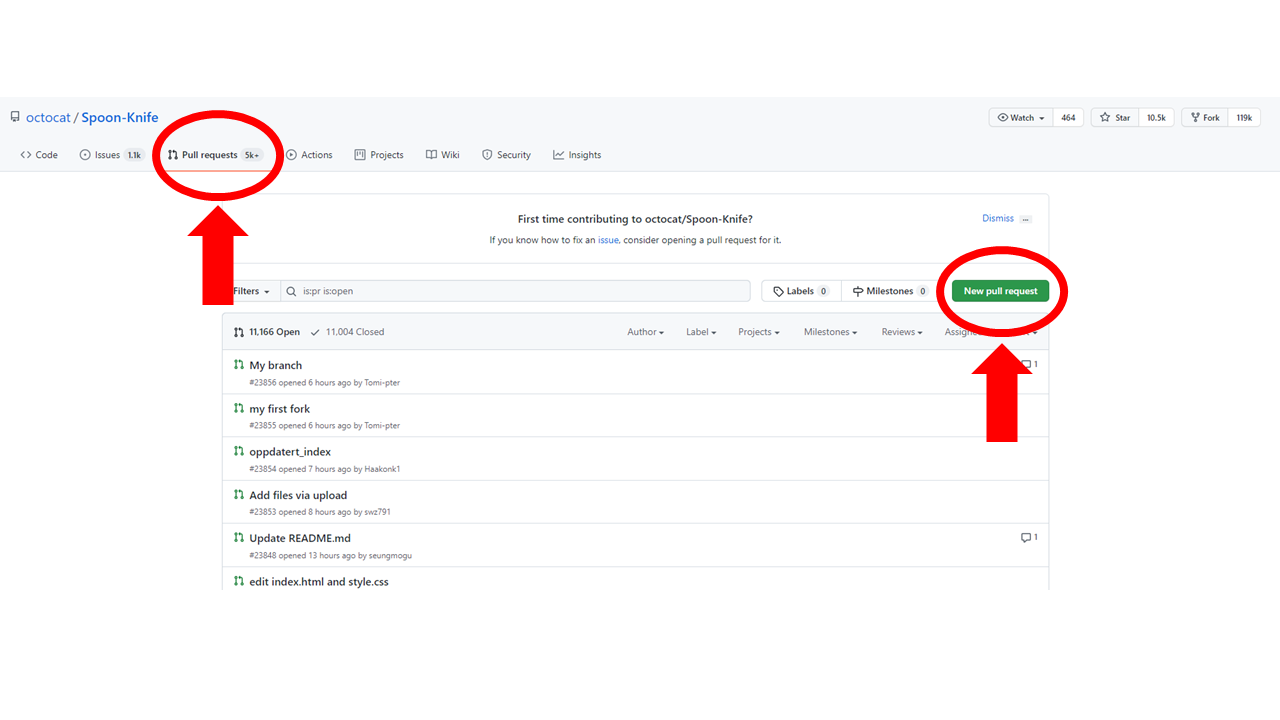
\includegraphics[width=1\linewidth]{img/github-04} 

}

\caption{Pull request}\label{fig:github04}
\end{figure}

Once everyone is happy with the proposed changes, you are ready to merge the pull request. If there are no merge conflicts, you will see a `Merge pull request' button.

\hypertarget{references}{%
\section{References}\label{references}}

\begin{itemize}
\tightlist
\item
  GitHub Community Forum: \url{https://github.community/}
\end{itemize}

\hypertarget{glossary}{%
\chapter{Glossary}\label{glossary}}

\begin{itemize}
\tightlist
\item
  \textbf{Branch}: A standalone history of commits existing on a repository.
\item
  \textbf{Clone}: Obtain a local copy of an existing repository.
\item
  \textbf{Command line}: The interface that allows us to give orders to our computer by typing commands instead of pointing and clicking. For anything that matters, shell, command line, and terminal are synonyms.
\item
  \textbf{Commit}: Save the current version of a file into the Git memory.
\item
  \textbf{Conflict}: A difference in the content of two repositories which prevents them from being synchronized.
\item
  \textbf{Fork}: Obtain a copy of an existing repository on your GitHub account.
\item
  \textbf{Hash}: Unique identifier for a commit.
\item
  \textbf{Local}: A file that is physically stored on your computer or a process that runs on your computer.
\item
  \textbf{Merge}: Integrate changes into a repository branch.
\item
  \textbf{Parent}: A directory that contains the current one.
\item
  \textbf{Pull}: Downloading changes from a remote repository to our local copy.
\item
  \textbf{Pull request}: Request to integrate changes from a fork into the original repository.
\item
  \textbf{Push}: Sending locally committed changes to a remote repository.
\item
  \textbf{Remote}: A version of a repository that is hosted elsewhere than your local copy, such as on a web server (like GitHub) or on a university network server.
\item
  \textbf{Root}: The parent directory of your file system. Sometimes the term ``root'' is used in a relative sense, e.g., to refer to the parent directory of a project rather than the parent directory of the whole file system.
\item
  \textbf{Shell}: The program that processes the commands we input in the command line. For anything that matters, shell, command line, and terminal are synonyms.
\item
  \textbf{Stage}: Add modified files to staging area, where they are ready to be committed.
\item
  \textbf{Terminal}: The window where you type commands for the computer. For anything that matters, shell, command line, and terminal are synonyms.
\item
  \textbf{Version control}: Any system that allows to track changes on a set of files.
\end{itemize}

  \bibliography{book.bib}

\end{document}
